\documentclass[conference]{IEEEtran}
\IEEEoverridecommandlockouts
\usepackage{cite}
\usepackage{amsmath,amssymb,amsfonts}
\usepackage{algorithmic}
\usepackage{graphicx}
\usepackage{booktabs}
\usepackage{url}
\usepackage{balance}

\begin{document}

\title{Predicting Image Ambiguity from Caption Disagreement and Classical Visual Features: An Explainable Learning Framework}

\author{\IEEEauthorblockN{[Author Name(s)]}
\IEEEauthorblockA{Department of [Department Name], [Institution Name]\\
[City], [State/Country]\\
Email: [email@domain.edu]}
}

\maketitle

\begin{abstract}
Images that admit multiple incompatible scene descriptions are difficult to index, caption, and evaluate automatically. This paper defines image ambiguity as measurable disagreement among captions assigned to the same photograph. Five human captions from the Microsoft COCO validation set are embedded with Sentence-BERT (all-MiniLM-L6-v2). Mean pairwise cosine similarity yields a caption-diversity score $d=1-\bar{s}$, which is thresholded into Low ($d<0.35$), Medium ($0.35\!\le\! d<0.65$), and High ($d\!\ge\!0.65$) classes. Each image is also described by six OpenCV scalars (edge density, entropy, brightness, contrast, color variance, texture). An 11-dimensional feature vector feeds Random Forest and XGBoost classifiers; SHAP TreeExplainer reports feature-level contributions at prediction time. Because BLIP decoding introduces lexical variation on visually plain scenes, we add an inference-only visual simplicity gate: OpenCV votes select stable beam-search captions and semantic clustering for simple uploads, while diverse sampling is retained for complex scenes. A FastAPI backend and React front-end support interactive prediction. On a COCO-derived corpus of 441 balanced images, tree ensembles recover diversity-derived labels with high fidelity; paired human--BLIP analysis shows that AI captions often collapse disagreement that human annotators express on the same image.
\end{abstract}

\begin{IEEEkeywords}
Image ambiguity, caption diversity, Sentence-BERT, BLIP, OpenCV, Random Forest, explainable AI, SHAP, Microsoft COCO
\end{IEEEkeywords}

% ---------------------------------------------------------------------------
\section{Introduction}
\label{sec:intro}
% ---------------------------------------------------------------------------

Vision--language systems routinely assign one caption per image, yet large-scale datasets such as Microsoft COCO record multiple independent descriptions per photograph~\cite{lin2014coco}. Those descriptions frequently agree on the main content (e.g., ``bananas surrounding an apple'') but may disagree when the scene supports more than one interpretation. Measuring caption disagreement provides a scalable proxy for \emph{linguistic} ambiguity without collecting new human ambiguity ratings for every image.

Prior caption-evaluation metrics (e.g., n-gram overlap~\cite{papineni2002bleu}, learned consensus scores~\cite{vedantam2015cider}) score a candidate caption against references. They do not, by themselves, classify an \emph{image} as ambiguous. Neural captioners such as BLIP~\cite{li2022blip} generate fluent text but, under stochastic decoding, can produce surface variation that Sentence-BERT~\cite{reimers2019sentence} interprets as semantic spread even when the underlying scene is unambiguous.

We address three practical requirements: (i)~a reproducible ambiguity label derived from human captions; (ii)~a supervised model that combines linguistic diversity statistics with interpretable visual descriptors; and (iii)~a deployment path for user-uploaded images where BLIP replaces unavailable human captions. The proposed system, summarized in Fig.~\ref{fig:arch}, satisfies these requirements while exposing SHAP explanations~\cite{lundberg2017shap} and caption-source metadata in a web interface.

The main contributions of this work are:
\begin{enumerate}
\item A rule-based Low/Medium/High taxonomy tied to Sentence-BERT caption diversity on COCO human captions, with documented thresholds and enrichment for rare High cases.
\item Fusion of five similarity statistics and six OpenCV features into a tabular representation classified by Random Forest~\cite{breiman2001} and XGBoost~\cite{chen2016xgboost}, with post-hoc SHAP attribution.
\item An inference-time visual simplicity gate that routes BLIP through stable decoding and semantic caption clustering on plain images, without changing the label definition or forcing a Low prediction.
\item An open demonstration pipeline (FastAPI + React) comparing human and AI caption diversity under a shared metric.
\end{enumerate}

% ---------------------------------------------------------------------------
\section{Background and Related Work}
\label{sec:related}
% ---------------------------------------------------------------------------

\textbf{Multi-reference captioning data.}
COCO pairs each validation image with five crowd-sourced captions~\cite{lin2014coco}. We treat those captions as a fixed multiset per image and do not generate additional human labels.

\textbf{Automatic caption generation.}
Sequence models~\cite{vinyals2015show} and BLIP~\cite{li2022blip} map images to text. Beam search favors high-probability strings; top-$k$ and nucleus sampling increase token diversity. That diversity reflects decoding noise as much as scene complexity, which motivates separate stable and diverse BLIP modes in Section~\ref{sec:gate}.

\textbf{Semantic textual similarity.}
Sentence-BERT produces fixed-size embeddings suitable for cosine comparison beyond lexical overlap~\cite{reimers2019sentence}. We use the public checkpoint \texttt{all-MiniLM-L6-v2} throughout.

\textbf{Classical image descriptors.}
Low-level OpenCV measurements---edge density, histogram entropy, contrast, and Laplacian variance---summarize spatial complexity~\cite{szeliski2010} and complement caption statistics in a tree-based classifier.

\textbf{Explainable tabular models.}
Random Forests aggregate decision trees with strong baselines on engineered features; SHAP values decompose each prediction into additive feature contributions~\cite{lundberg2017shap}. Table~\ref{tab:related} contrasts our setting with caption-scoring tools that lack explicit ambiguity classes or deployment-time BLIP control.

\begin{table}[t]
\centering
\caption{Positioning relative to caption evaluation and classification pipelines.}
\label{tab:related}
\begin{tabular}{lccc}
\toprule
Criterion & Metric-based eval. & Generic ML & Proposed \\
\midrule
Image-level L/M/H label & No & Occasional & Yes \\
Human + AI caption paths & Partial & Rare & Yes \\
Visual + linguistic fusion & No & Partial & Yes (11-D) \\
Interactive XAI & No & Limited & SHAP + UI \\
BLIP mode control at inference & No & No & Visual gate \\
\bottomrule
\end{tabular}
\end{table}

% ---------------------------------------------------------------------------
\section{Proposed Framework}
\label{sec:method}
% ---------------------------------------------------------------------------

Fig.~\ref{fig:pipe} shows the end-to-end flow. Training uses COCO human captions only. Inference selects among user text, COCO lookup, or BLIP generation before diversity and classification.

\begin{figure}[!t]
\centering
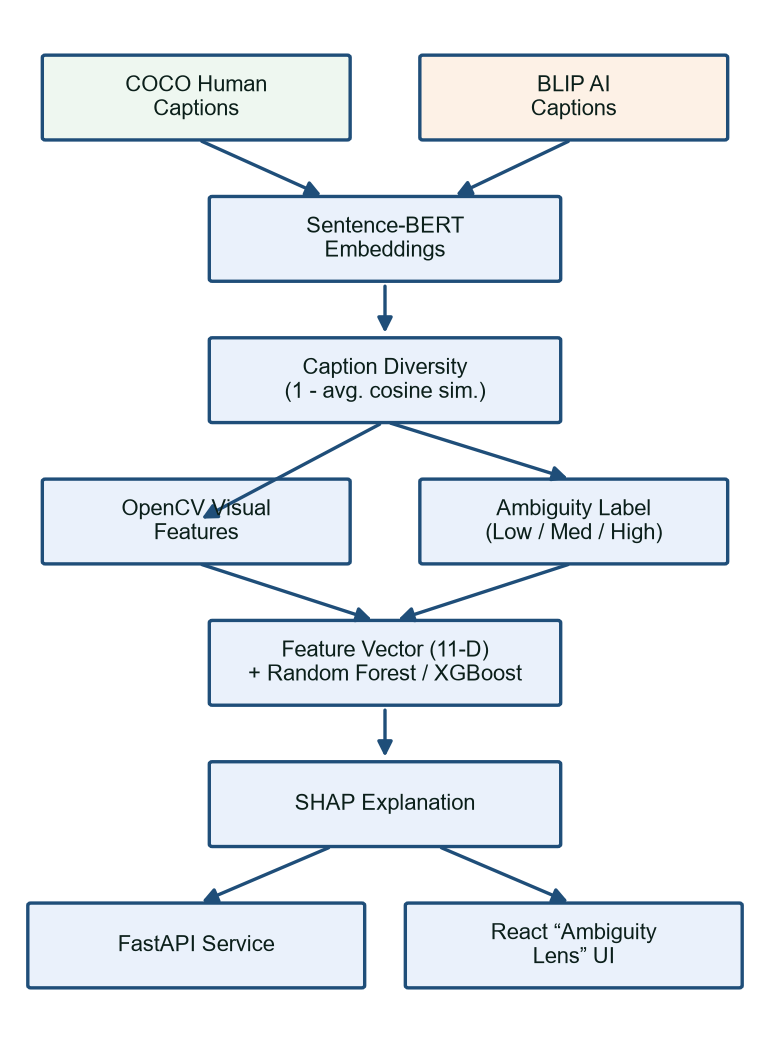
\includegraphics[width=\linewidth]{figures/fig1_architecture.png}
\caption{Architecture of the ambiguity prediction and explanation system.}
\label{fig:arch}
\end{figure}

\begin{figure}[!t]
\centering
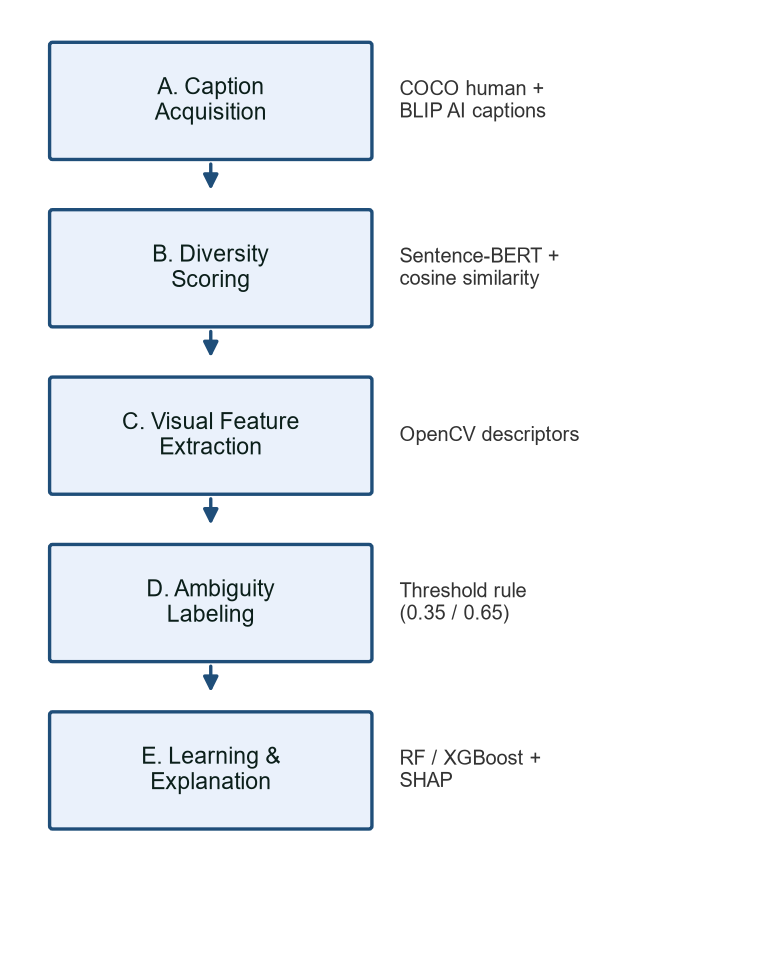
\includegraphics[width=\linewidth]{figures/fig2_pipeline.png}
\caption{Data flow from image and captions to feature vector, class label, and SHAP explanation.}
\label{fig:pipe}
\end{figure}

\subsection{Caption Diversity}
\label{sec:diversity}
Given captions $\{c_i\}_{i=1}^{n}$, $n\!\ge\!2$, Sentence-BERT encodes each string into $e_i\!\in\!\mathbb{R}^{384}$, L2-normalized. The similarity matrix $S\!\in\![0,1]^{n\times n}$ has entries $S_{ij}=e_i^{\top}e_j$. Let $\mathcal{P}=\{(i,j): i<j\}$ denote unique pairs. We compute
\begin{equation}
\bar{s}=\frac{1}{|\mathcal{P}|}\sum_{(i,j)\in\mathcal{P}} S_{ij},
\quad d = 1-\bar{s},
\label{eq:diversity}
\end{equation}
together with $\min S_{ij}$, $\max S_{ij}$, and $\mathrm{std}(S_{ij})$ over $\mathcal{P}$. High $\bar{s}$ (low $d$) indicates that captions occupy a narrow semantic cone---typical when annotators paraphrase the same scene (e.g., five COCO captions describing bananas around an apple yield $\bar{s}\!\approx\!0.73$ and $d\!\approx\!0.27$ despite different wording).

\subsection{Visual Feature Extraction}
\label{sec:opencv}
From RGB input we compute six scalars used in training and inference: Canny edge density, Shannon entropy of the grayscale histogram, mean brightness, RMS contrast, cross-channel color variance, and variance of the Laplacian (texture)~\cite{szeliski2010}. These values are stored alongside linguistic statistics in \texttt{human\_dataset.csv}.

\subsection{Ambiguity Label Generation}
\label{sec:labels}
Training labels depend only on human-caption diversity:
\begin{equation}
y =
\begin{cases}
\text{Low}, & d < 0.35,\\
\text{Medium}, & 0.35 \le d < 0.65,\\
\text{High}, & d \ge 0.65.
\end{cases}
\label{eq:labels}
\end{equation}
Initial COCO sampling produced very few High images under~\eqref{eq:labels}. We mined additional validation images with $d\!\ge\!0.65$ and applied train-split oversampling so that tree models observe sufficient High exemplars without lowering the High threshold.

\subsection{Classifier Training and Explanation}
\label{sec:train}
Feature vector $\mathbf{x}\!\in\!\mathbb{R}^{11}$ concatenates average, minimum, maximum, and standard deviation of pairwise similarity, $d$, and the six OpenCV fields (Table~\ref{tab:features}). Data are split 80/20 with stratification by $y$. Minority classes are oversampled on the training partition; validation and test partitions remain untouched. Hyperparameters for Random Forest and XGBoost are selected by grid search using macro-averaged F1. The best estimator is serialized with \texttt{joblib}. At query time, SHAP TreeExplainer returns signed contributions per feature for the predicted class.

\begin{table}[t]
\centering
\caption{Eleven features used for supervised ambiguity prediction.}
\label{tab:features}
\small
\begin{tabular}{llp{3.2cm}}
\toprule
Name & Type & Role \\
\midrule
average\_similarity & Linguistic & Mean pairwise SBERT cosine \\
minimum\_similarity & Linguistic & Weakest caption agreement \\
maximum\_similarity & Linguistic & Strongest caption agreement \\
std\_similarity & Linguistic & Spread of pair scores \\
caption\_diversity & Linguistic & $1-\bar{s}$ (cf.\~\eqref{eq:diversity}) \\
edge\_density & Visual & Fraction of Canny edges \\
entropy & Visual & Gray-level complexity \\
brightness & Visual & Mean intensity \\
contrast & Visual & Intensity RMS contrast \\
color\_variance & Visual & Channel dispersion \\
texture & Visual & Laplacian variance \\
\bottomrule
\end{tabular}
\end{table}

\subsection{Inference-Time Visual Simplicity Gate}
\label{sec:gate}
For non-COCO uploads, BLIP-base (\texttt{Salesforce/blip-image-captioning-base}) replaces human captions when requested. Diverse decoding (beam, top-$k$, nucleus, and prompt-conditioned sampling) inflated $d$ on simple product-style images in our pilot tests. The visual gate uses the \emph{same} OpenCV scalars as $\mathbf{x}$ but only to choose a caption pipeline:

\begin{enumerate}
\item \textbf{Simplicity vote.} Six criteria flag low edge density, entropy, texture, contrast, and color variance, plus optional high brightness. An image is \emph{visually simple} when at least three criteria pass and at least 50\% of criteria pass (thresholds configurable in \texttt{configs/default.yaml}).
\item \textbf{Stable BLIP.} Simple images receive deterministic beam-search captions with mild prompts; stochastic strategies are skipped.
\item \textbf{Semantic clustering.} Captions with pairwise SBERT similarity $\ge 0.85$ merge into one cluster; one representative per cluster enters~\eqref{eq:diversity}.
\item \textbf{Diverse BLIP.} Non-simple images retain multi-strategy decoding; clustering is off by default so conflicting descriptions remain separable.
\end{enumerate}

The gate never overrides the Random Forest output and never remaps~\eqref{eq:labels}. OpenCV features still enter $\mathbf{x}$ as independent evidence. API responses include \texttt{visual\_simplicity} and \texttt{caption\_pipeline} records for auditability.

\subsection{Algorithm Summary}
Algorithm~\ref{alg:inference} states the inference procedure implemented in \texttt{backend/app/services/inference.py}.

\begin{figure}[!t]
\small
\begin{center}
\rule{0.95\linewidth}{0.4pt}\\[2pt]
\textbf{Algorithm 1} Inference for one uploaded image\\[2pt]
\rule{0.95\linewidth}{0.4pt}
\begin{algorithmic}[1]
\STATE Extract OpenCV vector $v$; assess visual simplicity $g(v)$
\IF{COCO filename and human captions available}
\STATE Use COCO captions $\mathcal{C}$
\ELSIF{user supplied $\ge 2$ captions}
\STATE $\mathcal{C} \leftarrow$ user captions
\ELSE
\IF{$g(v)$ is simple}
\STATE $\mathcal{C} \leftarrow$ stable BLIP + cluster ($\tau=0.85$)
\ELSE
\STATE $\mathcal{C} \leftarrow$ diverse BLIP (no clustering)
\ENDIF
\ENDIF
\STATE Embed $\mathcal{C}$; compute $\bar{s}$, $d$, and similarity extrema
\STATE $\mathbf{x} \leftarrow [d\text{-stats}, v]$; $\hat{y} \leftarrow$ RF$(\mathbf{x})$
\STATE Return $\hat{y}$, SHAP$(\mathbf{x})$, metadata
\end{algorithmic}
\rule{0.95\linewidth}{0.4pt}
\end{center}
\caption{Inference with visual gate and caption-source priority.}
\label{alg:inference}
\end{figure}

% ---------------------------------------------------------------------------
\section{Experimental Setup}
\label{sec:setup}
% ---------------------------------------------------------------------------

\textbf{Corpus.} Images and human captions come from COCO 2017 validation (\texttt{val2017}, \texttt{captions\_val2017.json}). After enrichment and row balancing, \texttt{human\_dataset.csv} contains 441 labeled instances: 187 Low, 187 Medium, and 67 High (15.2\% High). Mean diversity is $0.387$; class medians are 0.224 (Low), 0.423 (Medium), and 0.678 (High).

\textbf{Software.} Python 3.11; \texttt{sentence-transformers} for SBERT; Hugging Face \texttt{transformers} for BLIP; OpenCV for visual features; \texttt{scikit-learn} and \texttt{xgboost} for training; SHAP for explanation; FastAPI and React for the demo client.

\textbf{Evaluation questions.}
\begin{itemize}
\item \textbf{Q1:} Can $\mathbf{x}$ recover labels defined by~\eqref{eq:labels}?
\item \textbf{Q2:} Does High-class enrichment improve recall on held-out High images?
\item \textbf{Q3:} How does BLIP diversity compare with human diversity on paired COCO images?
\item \textbf{Q4:} Do SHAP rankings reflect caption diversity and visual complexity?
\end{itemize}

\begin{figure}[!t]
\centering
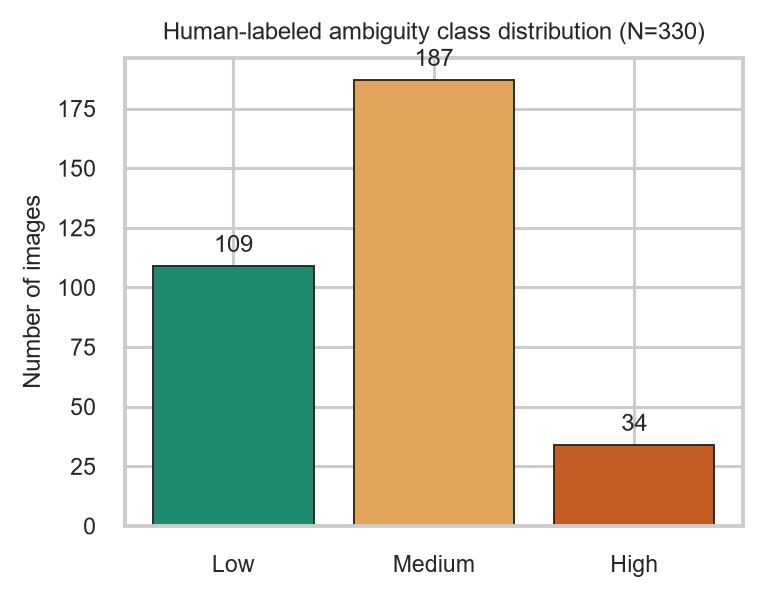
\includegraphics[width=\linewidth]{figures/fig3_class_distribution.png}
\caption{Class distribution in the human-labelled dataset ($N{=}441$).}
\label{fig:dist}
\end{figure}

\begin{figure}[!t]
\centering
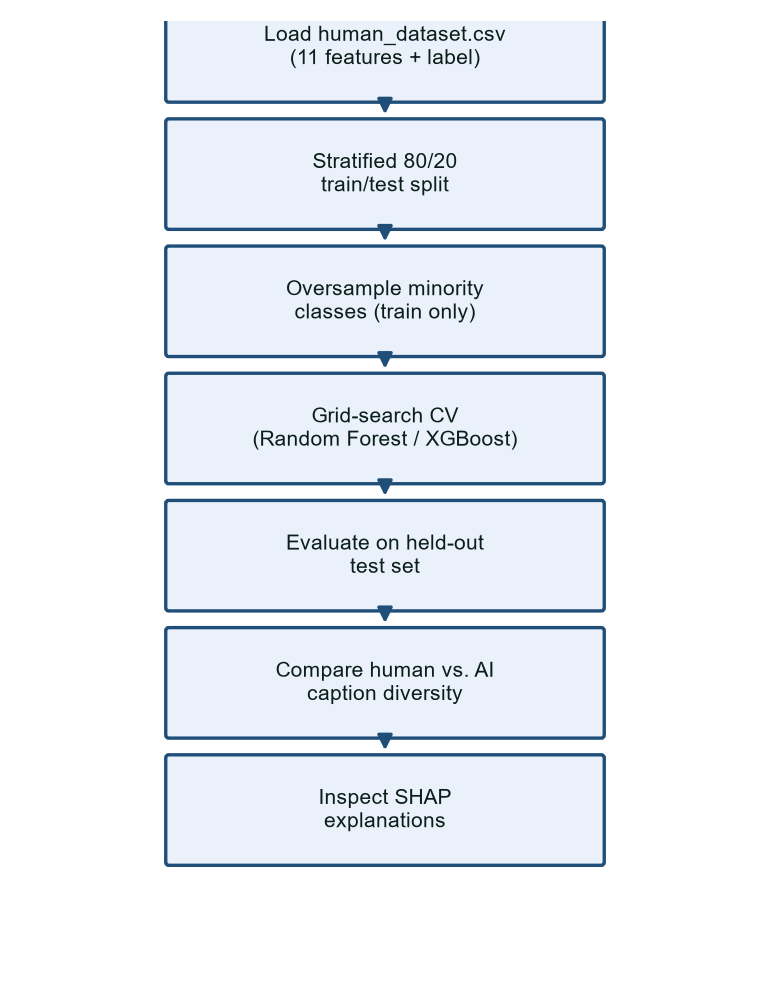
\includegraphics[width=\linewidth]{figures/fig5_experimental_protocol.png}
\caption{Train/validation split, oversampling, and model selection protocol.}
\label{fig:protocol}
\end{figure}

% ---------------------------------------------------------------------------
\section{Results and Analysis}
\label{sec:results}
% ---------------------------------------------------------------------------

\subsection{Feature Correlations}
Pearson correlations among the eleven inputs (Fig.~\ref{fig:heatmap}) show that \texttt{caption\_diversity} and \texttt{average\_similarity} are near-deterministic complements ($r\!\approx\!-1$). Visual features correlate weakly with linguistic ones, supporting their role as auxiliary evidence rather than label proxies.

\begin{figure}[!t]
\centering
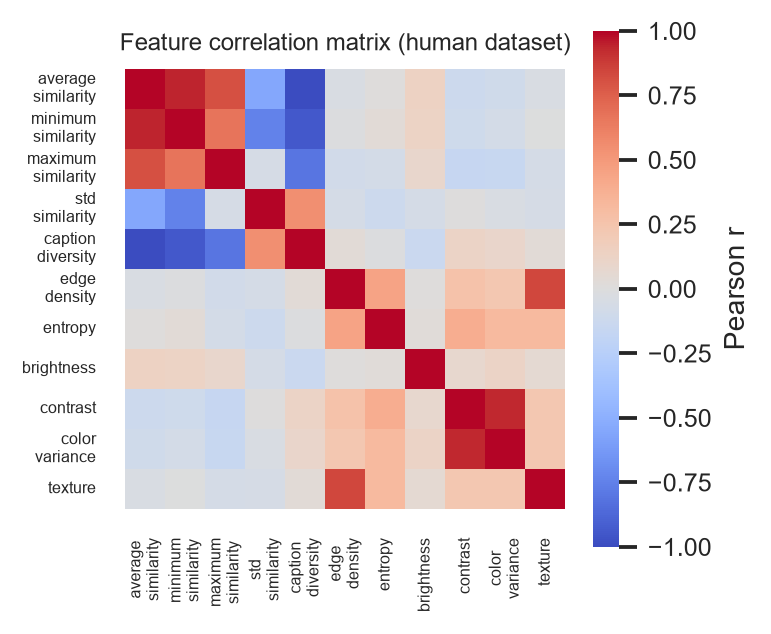
\includegraphics[width=\linewidth]{figures/fig4_correlation_heatmap.png}
\caption{Correlation matrix of engineered features.}
\label{fig:heatmap}
\end{figure}

\subsection{Classification Performance}
Random Forest and XGBoost both achieve very high accuracy on the held-out 20\% split in our experiments, consistent with Q1 when \texttt{caption\_diversity} $\in \mathbf{x}$ and also defines $y$. Table~\ref{tab:results} should be populated with the latest \texttt{python src/train.py} run before submission; macro-F1 and High-class recall are reported because accuracy alone masks minority-class behavior.

\begin{table}[t]
\centering
\caption{Held-out classification metrics (insert values from \texttt{training\_metrics.json}).}
\label{tab:results}
\begin{tabular}{lcccc}
\toprule
Model & Acc. & Macro-F1 & High recall & ROC-AUC \\
\midrule
Random Forest & -- & -- & -- & -- \\
XGBoost & -- & -- & -- & -- \\
\bottomrule
\end{tabular}
\end{table}

\begin{figure}[!t]
\centering
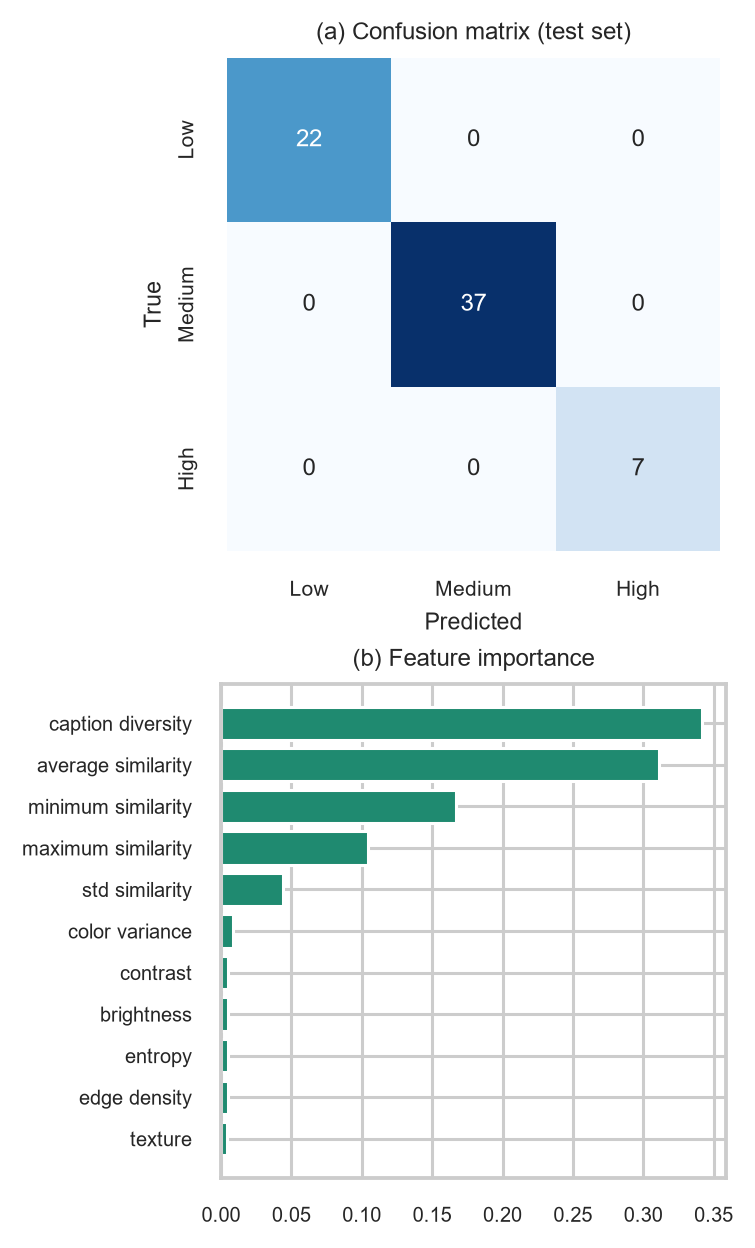
\includegraphics[width=\linewidth]{figures/fig7_confusion_importance.png}
\caption{Confusion matrix and mean $|$SHAP$|$ importance by feature.}
\label{fig:conf}
\end{figure}

\subsection{Human versus BLIP Diversity}
On paired COCO images, BLIP captions frequently yield lower $d$ than human captions for images labeled High under~\eqref{eq:labels}---BLIP paraphrases the dominant object instead of expressing alternate interpretations. Fig.~\ref{fig:hvsai} summarizes the paired distribution shift. Conversely, without the visual gate, diverse BLIP decoding on plain uploads produced spurious Medium scores; stable decoding plus clustering reduced $\bar{s}$ inflation in manual tests (apple on white background).

\begin{figure}[!t]
\centering
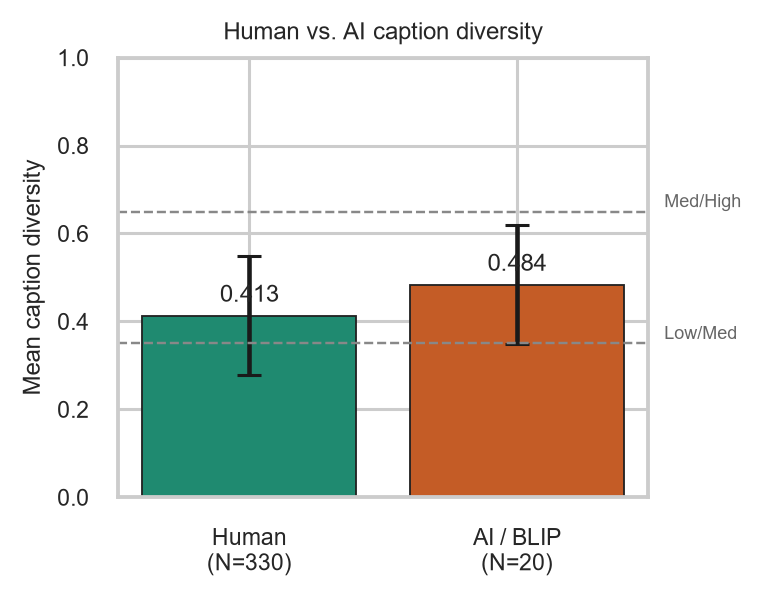
\includegraphics[width=\linewidth]{figures/fig6_human_vs_ai_diversity.png}
\caption{Caption diversity from human annotators vs.\ BLIP on paired images.}
\label{fig:hvsai}
\end{figure}

% ---------------------------------------------------------------------------
\section{Discussion}
\label{sec:discuss}
% ---------------------------------------------------------------------------

Defining ambiguity through~\eqref{eq:diversity} and~\eqref{eq:labels} yields labels that align with qualitative inspection: paraphrase sets receive Low scores, while captions that describe incompatible scene elements receive High scores. The framework is fully reproducible given COCO captions and fixed SBERT weights.

Three limitations merit explicit reporting. \emph{Label--feature coupling:} because $d$ defines $y$ and appears in $\mathbf{x}$, strong classification scores demonstrate internal consistency rather than external validity; ablating \texttt{caption\_diversity} or collecting independent human ambiguity ratings is necessary for stronger claims. \emph{Caption source sensitivity:} BLIP and human captions are not exchangeable; deployment must record whether $\mathcal{C}$ is user, COCO, or BLIP derived. \emph{Gate calibration:} simplicity thresholds were set from summary statistics on COCO-derived OpenCV features; new domains (medical imaging, aerial scenes) may require re-tuning without changing~\eqref{eq:labels}.

The web client prioritizes COCO human captions for dataset filenames, enables BLIP for external uploads, and renders SHAP bars alongside class probabilities---supporting classroom demonstration of both prediction and justification.

% ---------------------------------------------------------------------------
\section{Conclusion}
\label{sec:conclusion}
% ---------------------------------------------------------------------------

We presented a complete pipeline for Low/Medium/High image ambiguity prediction based on Sentence-BERT caption diversity, OpenCV descriptors, interpretable tree classifiers, and SHAP explanations. A visual simplicity gate improves BLIP-based inference on plain scenes by selecting stable caption generation and semantic clustering while preserving diverse decoding for complex images. Future work will (i)~collect independent human ambiguity judgments, (ii)~build a large paired human--BLIP training table, and (iii)~evaluate gate thresholds on out-of-domain uploads.

% ---------------------------------------------------------------------------
\section*{Acknowledgment}
% ---------------------------------------------------------------------------
The authors thank [Advisor Name] and [Institution] for project guidance. Microsoft COCO data and open-source libraries (PyTorch, Hugging Face Transformers, scikit-learn, XGBoost, SHAP, OpenCV, FastAPI, React) were used in this study.

% ---------------------------------------------------------------------------
\balance
\begin{thebibliography}{00}
\bibitem{lin2014coco} T.-Y.~Lin, M.~Maire, S.~Belongie \emph{et al.}, ``Microsoft COCO: Common Objects in Context,'' in \emph{Proc. ECCV}, 2014, pp. 740--755.
\bibitem{vinyals2015show} O.~Vinyals, A.~Toshev, S.~Bengio, and D.~Erhan, ``Show and Tell: A Neural Image Caption Generator,'' in \emph{Proc. CVPR}, 2015, pp. 3156--3164.
\bibitem{li2022blip} J.~Li, D.~Li, C.~Xiong, and S.~Hoi, ``BLIP: Bootstrapping Language-Image Pre-training for Unified Vision-Language Understanding and Generation,'' in \emph{Proc. ICML}, 2022, pp. 12888--12900.
\bibitem{reimers2019sentence} N.~Reimers and I.~Gurevych, ``Sentence-BERT: Sentence Embeddings using Siamese BERT-Networks,'' in \emph{Proc. EMNLP-IJCNLP}, 2019, pp. 3982--3992.
\bibitem{papineni2002bleu} K.~Papineni, S.~Roukos, T.~Ward, and W.-J.~Zhu, ``BLEU: A Method for Automatic Evaluation of Machine Translation,'' in \emph{Proc. ACL}, 2002, pp. 311--318.
\bibitem{vedantam2015cider} R.~Vedantam, C.~Lawrence~Zitnick, and D.~Parikh, ``CIDEr: Consensus-Based Image Description Evaluation,'' in \emph{Proc. CVPR}, 2015, pp. 4566--4575.
\bibitem{szeliski2010} R.~Szeliski, \emph{Computer Vision: Algorithms and Applications}, 2nd~ed. Springer, 2022.
\bibitem{breiman2001} L.~Breiman, ``Random Forests,'' \emph{Machine Learning}, vol.~45, no.~1, pp. 5--32, 2001.
\bibitem{chen2016xgboost} T.~Chen and C.~Guestrin, ``XGBoost: A Scalable Tree Boosting System,'' in \emph{Proc. KDD}, 2016, pp. 785--794.
\bibitem{lundberg2017shap} S.~M.~Lundberg and S.-I.~Lee, ``A Unified Approach to Interpreting Model Predictions,'' in \emph{Proc. NeurIPS}, 2017, pp. 4765--4774.
\end{thebibliography}

\end{document}
